\section{Theorie}
\label{sec:Theorie}

Der Doppler-Effekt beschreibt die Veränderung der Frequenz, wenn sich der Beobachter und eine Schallquelle relativ zu einander bewegen.
Bewegt sich die Quelle auf den Hörer zu, so wird die Grundfrequenz $\nu_0$ zu einer höheren Frequenz $\nu_{\text{kl}}$ verschoben.
Vergrößert sich der Abstand, reduziert sich die Frequenz zu $\nu_{\text{gr}}$.
Dabei gilt folgender mathematischer Zusammenhang
\begin{equation*}
    \nu_{\text{kl/gr}}=\frac{\nu_0}{1\mp \frac{v}{c}}\. .
\end{equation*}
Dieser Effekt wird in der Ultraschalltechnik verwendet, um z.B. die Geschwindigkeit von Blutströmungen zu ermitteln.
Wenn die Ultraschallwelle auf ein Blutkörper trifft, wird so die Frequenz $\nu_0$ verschoben.
Diese Verschiebung wird über die Formel
\begin{equation*}
    \bigtriangleup \nu=\nu_0 \frac{v}{c} (\cos{\alpha}+\cos{\beta}) 
\end{equation*}
beschrieben. Hierbei ist $v$ die Geschwindigkeit des Objektes, $c$ die Schallgeschwindigkeit und $\alpha$ und $\beta$ die Winkel zwischen Bewegungsrichtung und der 
Wellennormalen der ein- bzw. auslaufenden Welle.
Diese Messmethodik ist in \autoref{fig:Blutstrom} dargestellt. 
\begin{figure}
    \centering
    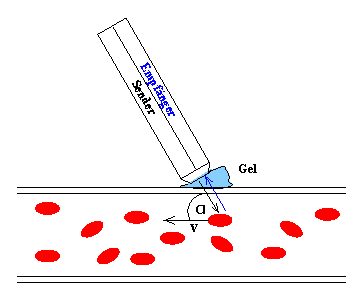
\includegraphics[width =6cm]{Blutstrom.pdf}
    \caption{Darstellung der Messung einer Blutstromgeschwingkeit mittels Doppler-Effekt\cite{apus3}.}
    \label{fig:Blutstrom}
\end{figure}
\begin{equation*}
    \bigtriangleup \nu=2\nu_0 \frac{v}{c} \cos{\alpha} 
\end{equation*}
folgt.
Als Erzeuger und Empfänger der Ultraschallwellen dient ein Piezokristall.